\documentclass[conference]{IEEEtran}
\IEEEoverridecommandlockouts
% The preceding line is only needed to identify funding in the first footnote. If that is unneeded, please comment it out.
\usepackage{cite}
\usepackage{amsmath,amssymb,amsfonts}
\usepackage{algorithmic}
\usepackage{graphicx}
\usepackage{textcomp}
\usepackage{xcolor}
\def\BibTeX{{\rm B\kern-.05em{\sc i\kern-.025em b}\kern-.08em
    T\kern-.1667em\lower.7ex\hbox{E}\kern-.125emX}}
\begin{document}

\title{Estudo Experimental de Associações de Resistores e Efeito Joule\\
{\footnotesize Relatório de Laboratório}
}
\author{\IEEEauthorblockN{1\textsuperscript{st} Arthur Cadore Matuella Barcella}
    \IEEEauthorblockA{\textit{Departamento de Telecomunicações} \\
        \textit{Instituto Federal de Santa Catarina}\\
        São José, Brasil \\
        arthur.cmb@aluno.ifsc.edu.br}
    \and
    \IEEEauthorblockN{2\textsuperscript{nd} Faber Bernardo Junior}
    \IEEEauthorblockA{\textit{Departamento de Telecomunicações} \\
        \textit{Instituto Federal de Santa Catarina}\\
        São José, Brasil \\
        faber.b@aluno.ifsc.edu.br}
    \and
    \IEEEauthorblockN{3\textsuperscript{rd} Gabriel Luiz Espindola Pedro}
    \IEEEauthorblockA{\textit{Departamento de Telecomunicações} \\
        \textit{Instituto Federal de Santa Catarina}\\
        São José, Brasil \\
        gabriel.ep@aluno.ifsc.edu.br}
}

\maketitle

\begin{abstract}
    This document is a model and instructions for \LaTeX.
    This and the IEEEtran.cls file define the components of your paper [title, text, heads, etc.]. *CRITICAL: Do Not Use Symbols, Special Characters, Footnotes,
    or Math in Paper Title or Abstract.
\end{abstract}

\begin{IEEEkeywords}
    component, formatting, style, styling, insert
\end{IEEEkeywords}

\section{Introdução:}

% [COMENTARIO PROFESSOR] Aqui pode ser utilizado para iniciar o resumo
Este experimento tem como objetivo analisar o comportamento de associações de resistores em série e em paralelo, utilizando cinco resistores de $1 k\Omega$ e cinco de $1 M\Omega$. As medições serão realizadas em corrente contínua (CC), com o uso de multímetro e osciloscópio para observar as respostas dos circuitos.

A compreensão de como a disposição dos resistores influencia a resistência total de um circuito é essencial na eletrônica. Além disso, este experimento proporciona experiência prática com instrumentos de medição e desenvolve habilidades em análise experimental.

\section{Revisão de literatura:}

As associações de resistores são fundamentais em circuitos elétricos.
Em associação série, a resistência equivalente é dada pela soma dos valores individuais.% [COMENTARIO PROFESSOR] adicionar referência
Já em associação paralelo, a resistência equivalente é obtida pela soma dos inversos das resistências individuais.

Em corrente alternada (CA), além da resistência,
fatores como capacitâncias e indutâncias parasitas podem influenciar o comportamento do circuito, especialmente em altas frequências. % [COMENTARIO PROFESSOR] adicionar referência
O multímetro é utilizado para medir resistência, tensão e corrente em CC, enquanto o osciloscópio permite visualizar formas de onda e analisar a resposta dinâmica dos circuitos.

Esta seção revisa os conceitos teóricos fundamentais para a análise experimental, reforçando a importância de compreender as associações resistivas e as limitações práticas dos instrumentos de medição.

\section{Resistores Comerciais}

Em eletrônica, não é viável fabricar resistores com qualquer valor numérico de resistência. Por isso, a indústria adota séries padronizadas de resistores, como as séries E12, E24, entre outras. % [COMENTARIO PROFESSOR] adicionar referência
Essas séries definem um conjunto finito de valores nominais por década, de forma que seja possível cobrir uma ampla faixa de resistências com precisão adequada para a maioria das aplicações.

O uso de resistores comerciais padronizados é essencial para facilitar a fabricação em escala, reduzir custos, garantir intercambialidade entre componentes e assegurar a reposição em projetos práticos. No entanto, nem sempre é possível encontrar exatamente o valor desejado entre os disponíveis na série padrão. % [COMENTARIO PROFESSOR] qual seria o impedimento?

Para contornar essa limitação, é comum combinar resistores em série e/ou paralelo para obter valores de resistência equivalentes que não estejam disponíveis diretamente no mercado.
Assim, qualquer valor de resistência pode ser aproximado com boa precisão por meio de associações de resistores comerciais,% [COMENTARIO PROFESSOR] e o erro na medida? "tolerancia"
o que reforça a importância de entender e aplicar corretamente os princípios dessas associações em projetos eletrônicos.

\subsection{Série E12} % [COMENTARIO PROFESSOR] o que significa essa notação/codificação? tem uma referencia teorica? 

A série E12 é uma das mais comuns e contempla valores padronizados de resistores amplamente utilizados em aplicações gerais. As figuras % [COMENTARIO PROFESSOR] usar \autoref
a seguir ilustram como os resistores dessa série podem ser combinados em série e paralelo, destacando os efeitos dessas associações na resistência equivalente.% [COMENTARIO PROFESSOR] o que significa a cor e o gradiente


\begin{figure}[htbp]
    \centering
    \caption{Matriz de resistores em série E12}
    \label{fig:matriz_serie_e12}
    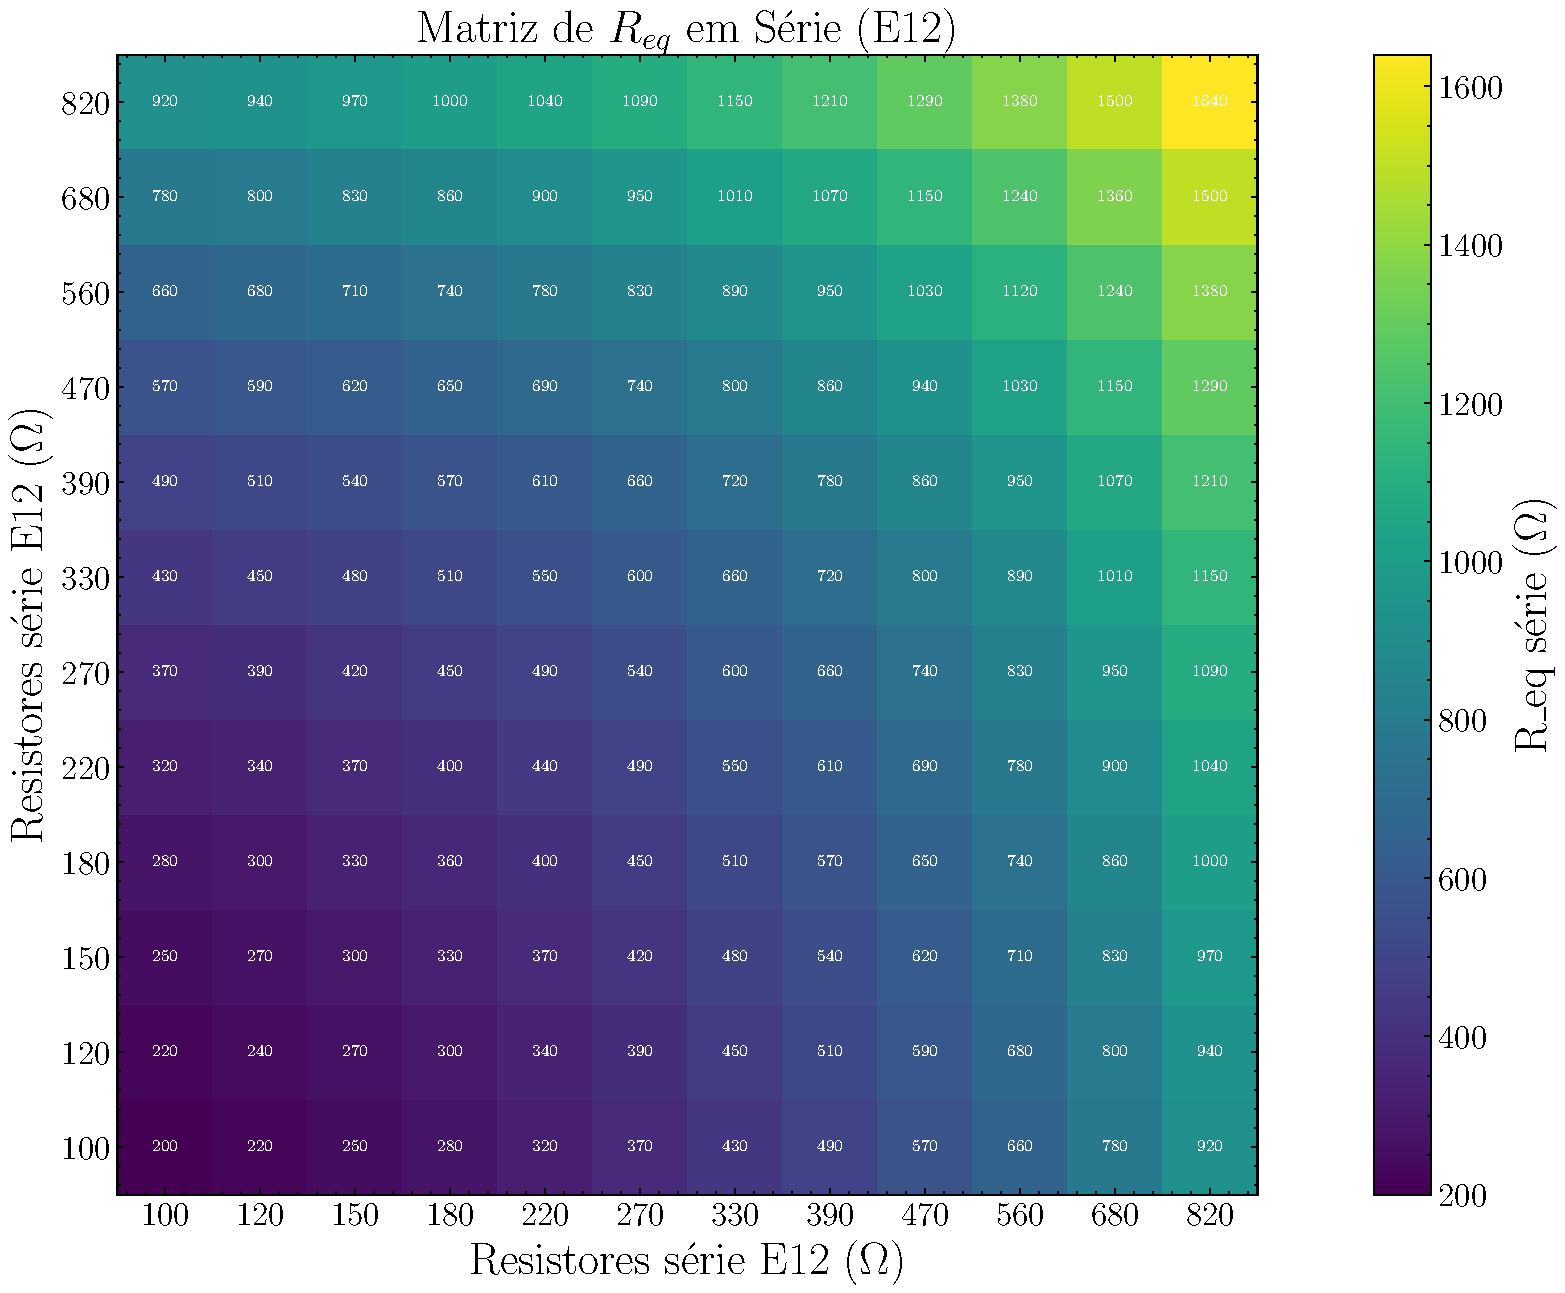
\includegraphics[width=0.8\linewidth]{figures/matriz_serie_e12.pdf}
\end{figure}

\begin{figure}[htbp]
    \centering
    \caption{Matriz de resistores em paralelo E12}
    \label{fig:matriz_paralelo_e12}
    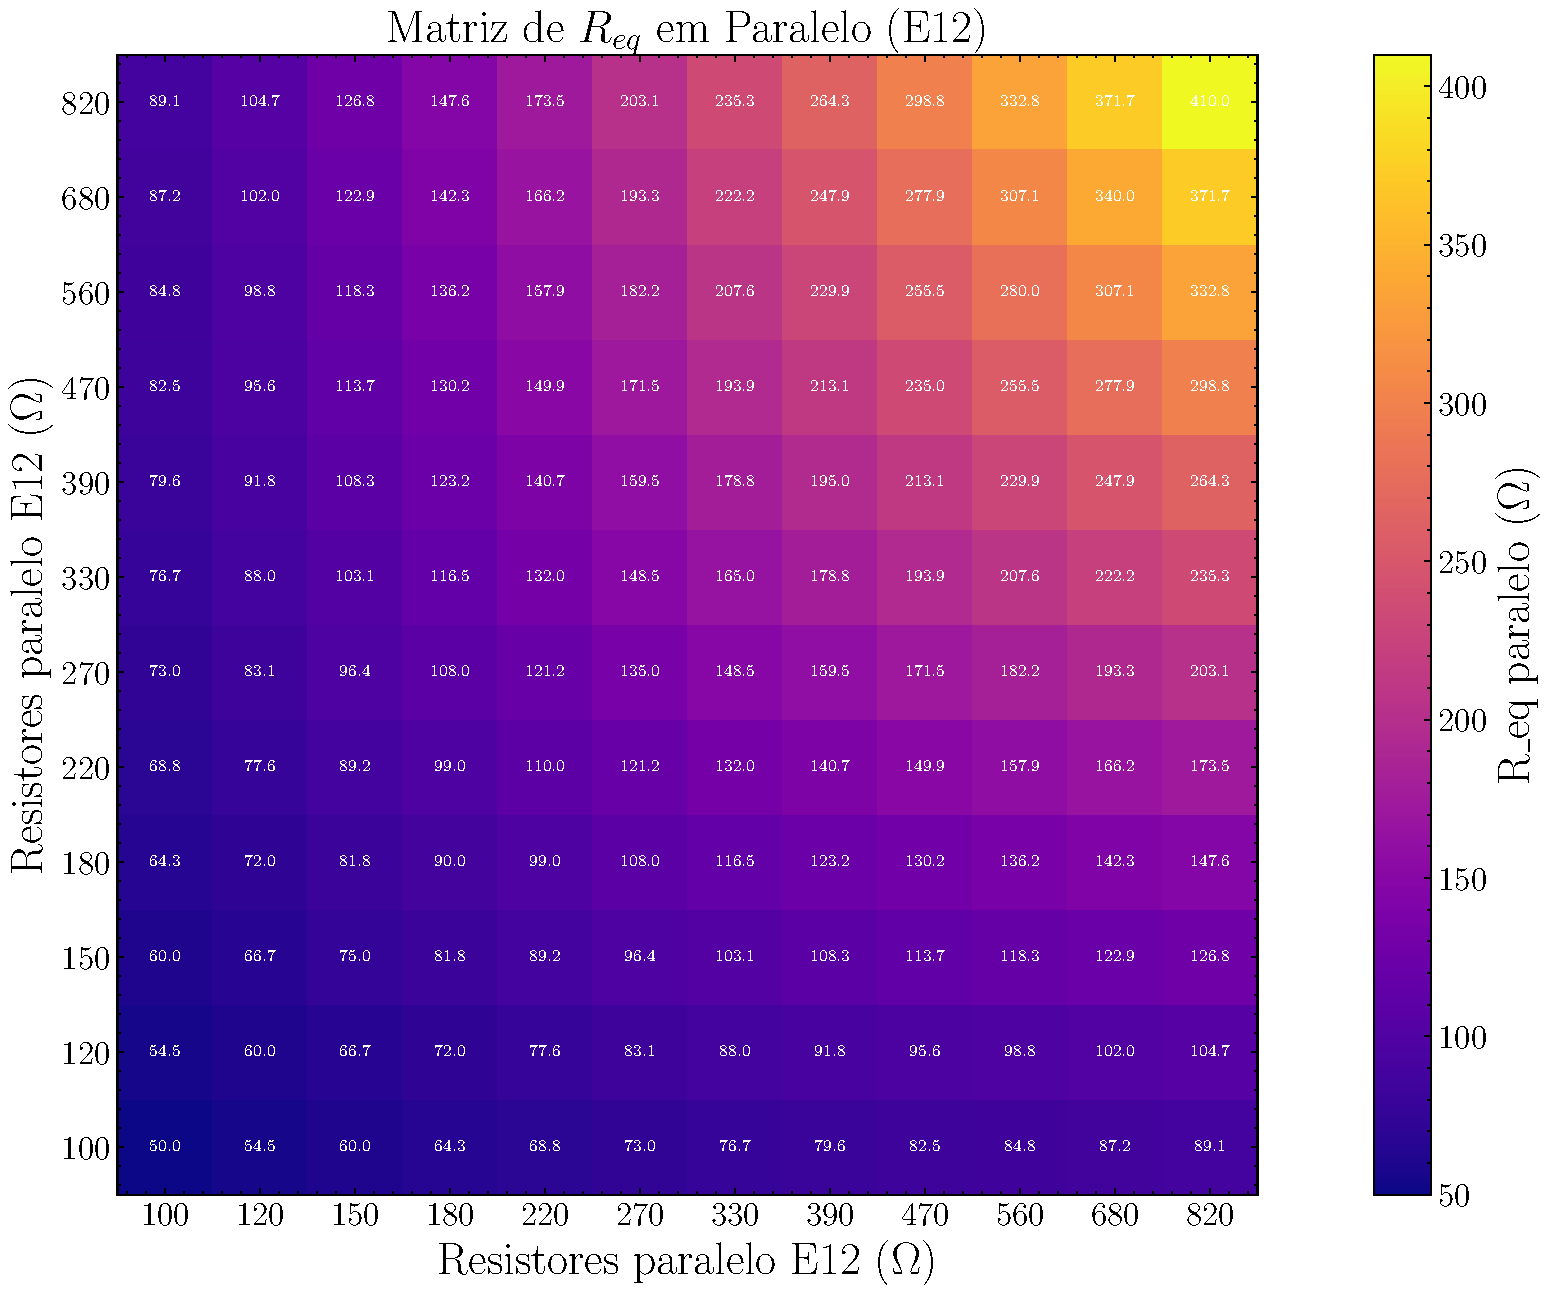
\includegraphics[width=0.8\linewidth]{figures/matriz_paralelo_e12.pdf}
\end{figure}

A associação em série resulta em uma resistência total maior, enquanto a associação em paralelo reduz a resistência equivalente.

\subsection{Série E24}% [COMENTARIO PROFESSOR] o que significa essa notação/codificação? tem uma referencia teorica? 

A série E24 oferece maior granularidade de valores comerciais, permitindo combinações ainda mais precisas para projetos eletrônicos. As associações possíveis são exemplificadas nas figuras a seguir:
\begin{figure}[htbp]
    \centering
    \caption{Matriz de resistores em série E24}
    \label{fig:matriz_serie_e24}
    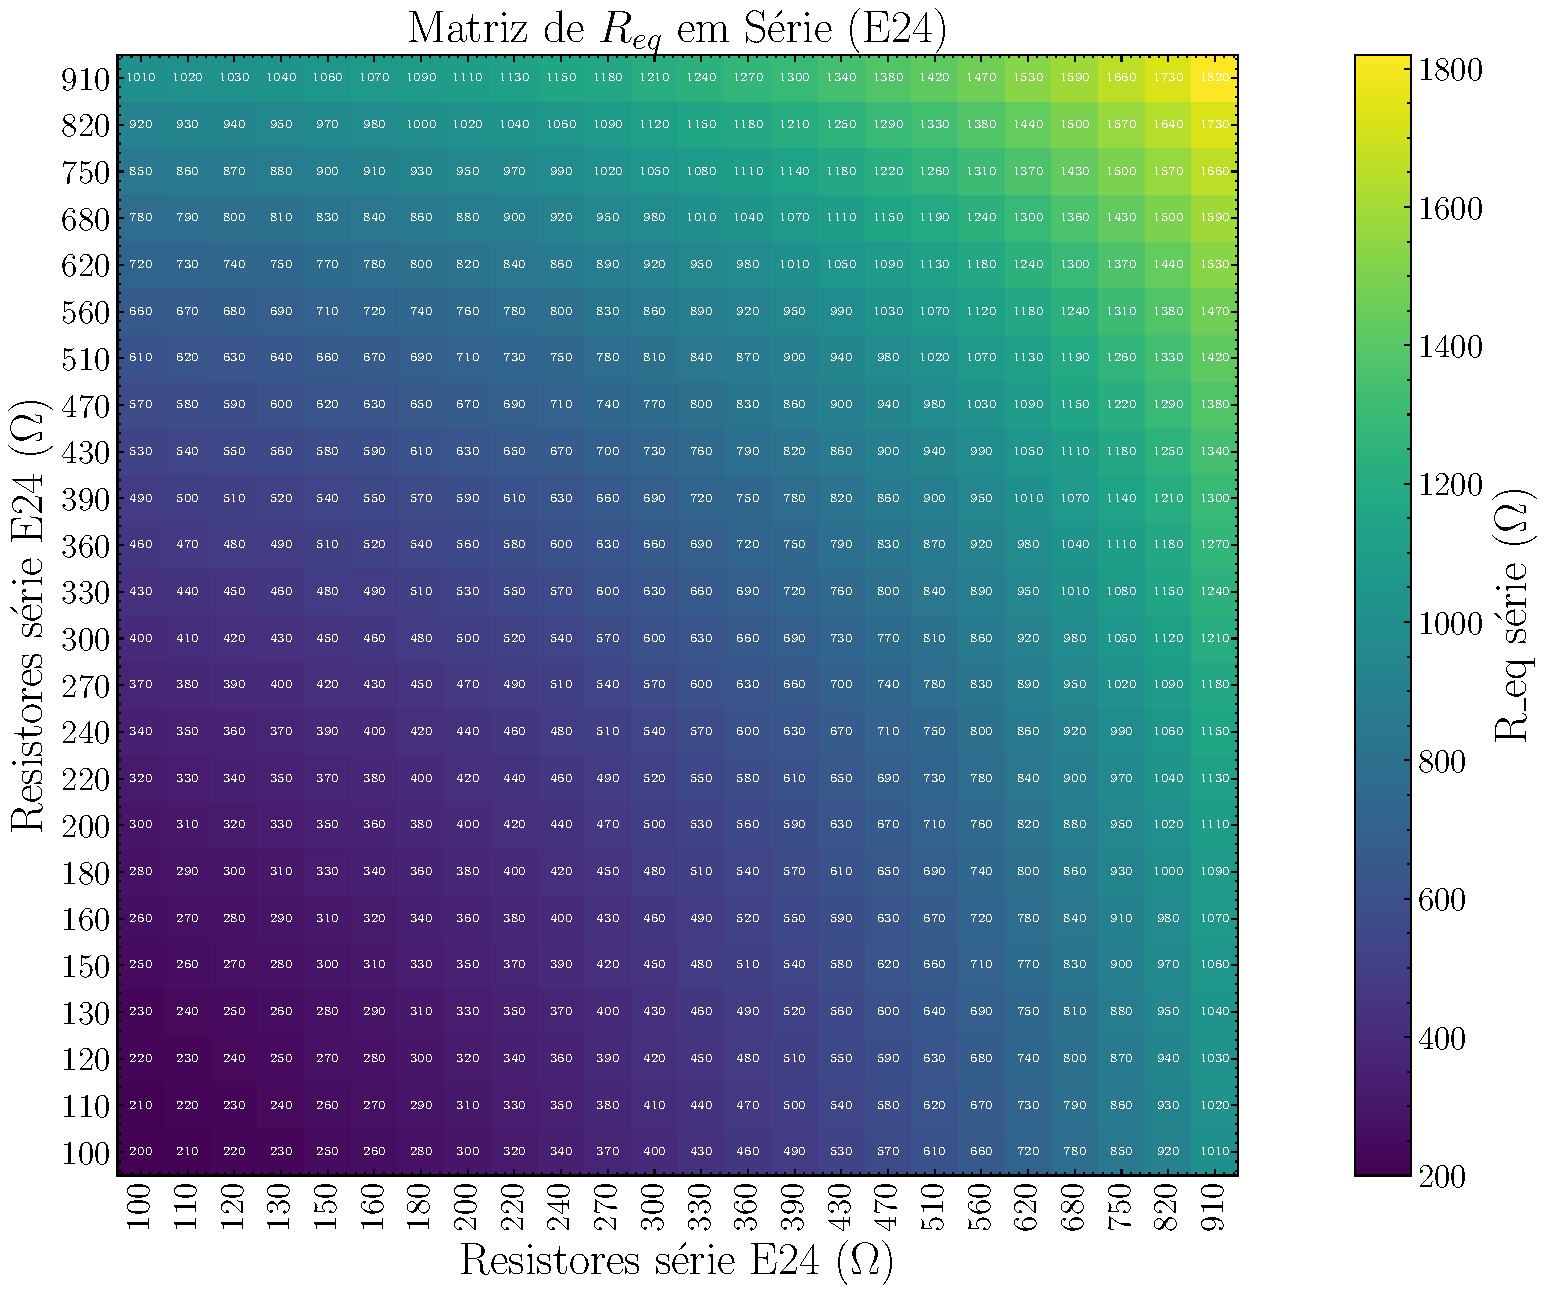
\includegraphics[width=0.8\linewidth]{figures/matriz_serie_e24.pdf}
\end{figure}

\begin{figure}[htbp]
    \centering
    \caption{Matriz de resistores em paralelo E24}
    \label{fig:matriz_paralelo_e24}
    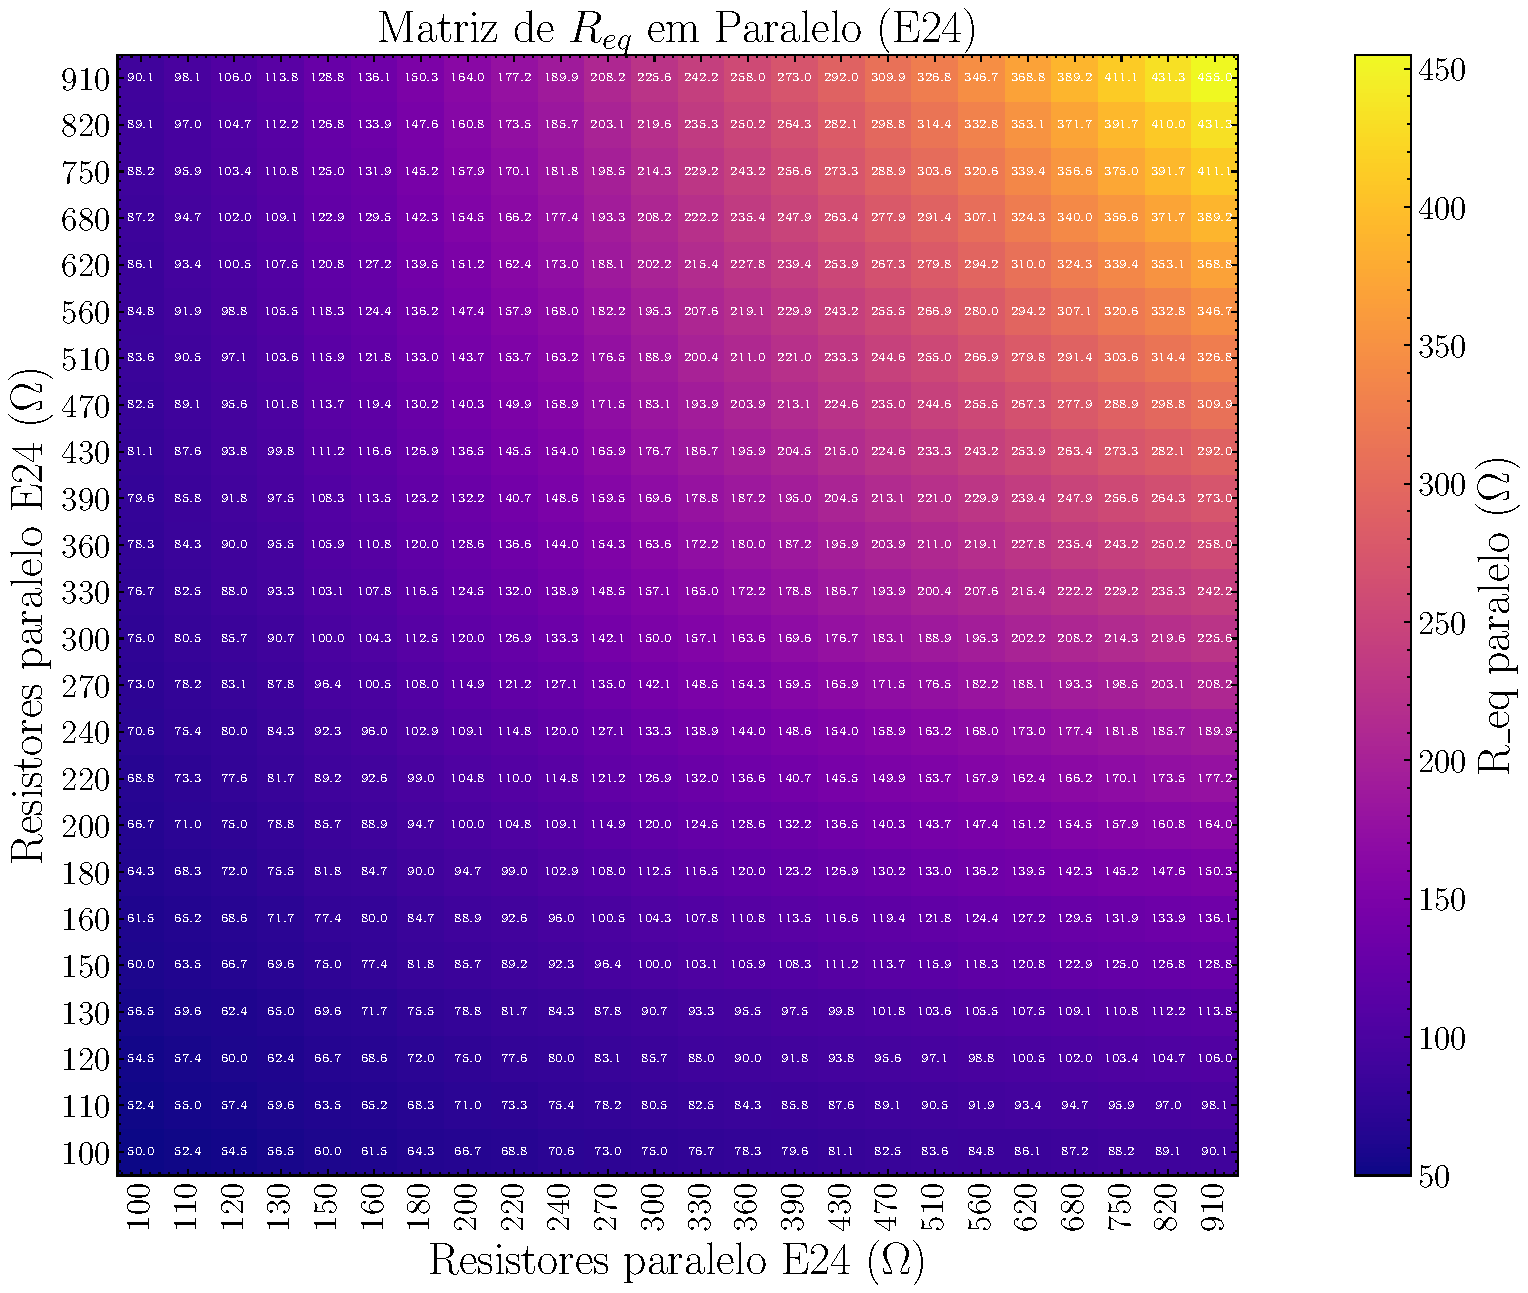
\includegraphics[width=0.8\linewidth]{figures/matriz_paralelo_e24.pdf}
\end{figure}


Essas associações demonstram como a escolha da série influencia a flexibilidade de valores alcançáveis em um projeto.



\section{Materiais e métodos:}

\begin{itemize}
    \item 10 resistores de $1k\Omega$ % [COMENTARIO PROFESSOR] e a tolerrancia (erro na leitura real das medidas)
          % [COMENTARIO PROFESSOR] erro de leitura das medidas que podemos ter ou aceitar nos resistores
    \item 10 resistores de $1M\Omega$
    \item Fonte de alimentação CC
    \item Multímetro digital
    \item Protoboard e cabos
    \item Resistor de aquecimento 1000W (220VAC) para simulação do efeito Joule
\end{itemize}

Foram montados circuitos com resistores em série, paralelo e mista. As medições de resistência, tensão e corrente foram realizadas com o multímetro digital. O protoboard facilita a montagem dos circuitos sem a necessidade de solda.

Para simular o efeito Joule, foi utilizado um resistor de aquecimento 1000W (220VAC) submerso em 500mL de água, com a temperatura ambiente de 25°C, e foi monitorada a temperatura da água ao longo do tempo até a temperatura de evaporação.

% [COMENTARIO PROFESSOR] adicionar fotos das montagens

\section{Associação de resistores:}

\subsection{Distribuição normal dos valores medidos:}

A análise estatística dos valores medidos permite determinar a média, desvio padrão e erro médio dos resistores:

Média

\begin{equation}
    R = \frac{1}{n} \sum_{i=1}^{n} R_i,
\end{equation}

\noindent
Onde $R$ é a média $n$ o número de resistores.

Desvio padrão:

\begin{equation}
    \sigma = \sqrt{\frac{1}{n-1} \sum_{i=1}^{n} (R_i - R)^2},
\end{equation}

\noindent
Onde $sigma$ representa a dispersão dos valores em relação à média.

Erro médio

\begin{equation}
    \Delta R = \frac{\sigma}{\sqrt{n}}, % [COMENTARIO PROFESSOR] deveira ser \sigma_n não \Delta R
\end{equation}

\noindent
Onde $\Delta R$ é o erro médio $sigma$ é o desvio padrão $n$ é o número de resistores.

\begin{figure}[htbp]
    \centering
    \caption{Distribuição normal dos valores medidos}
    \label{fig:plot_hist_1k}
    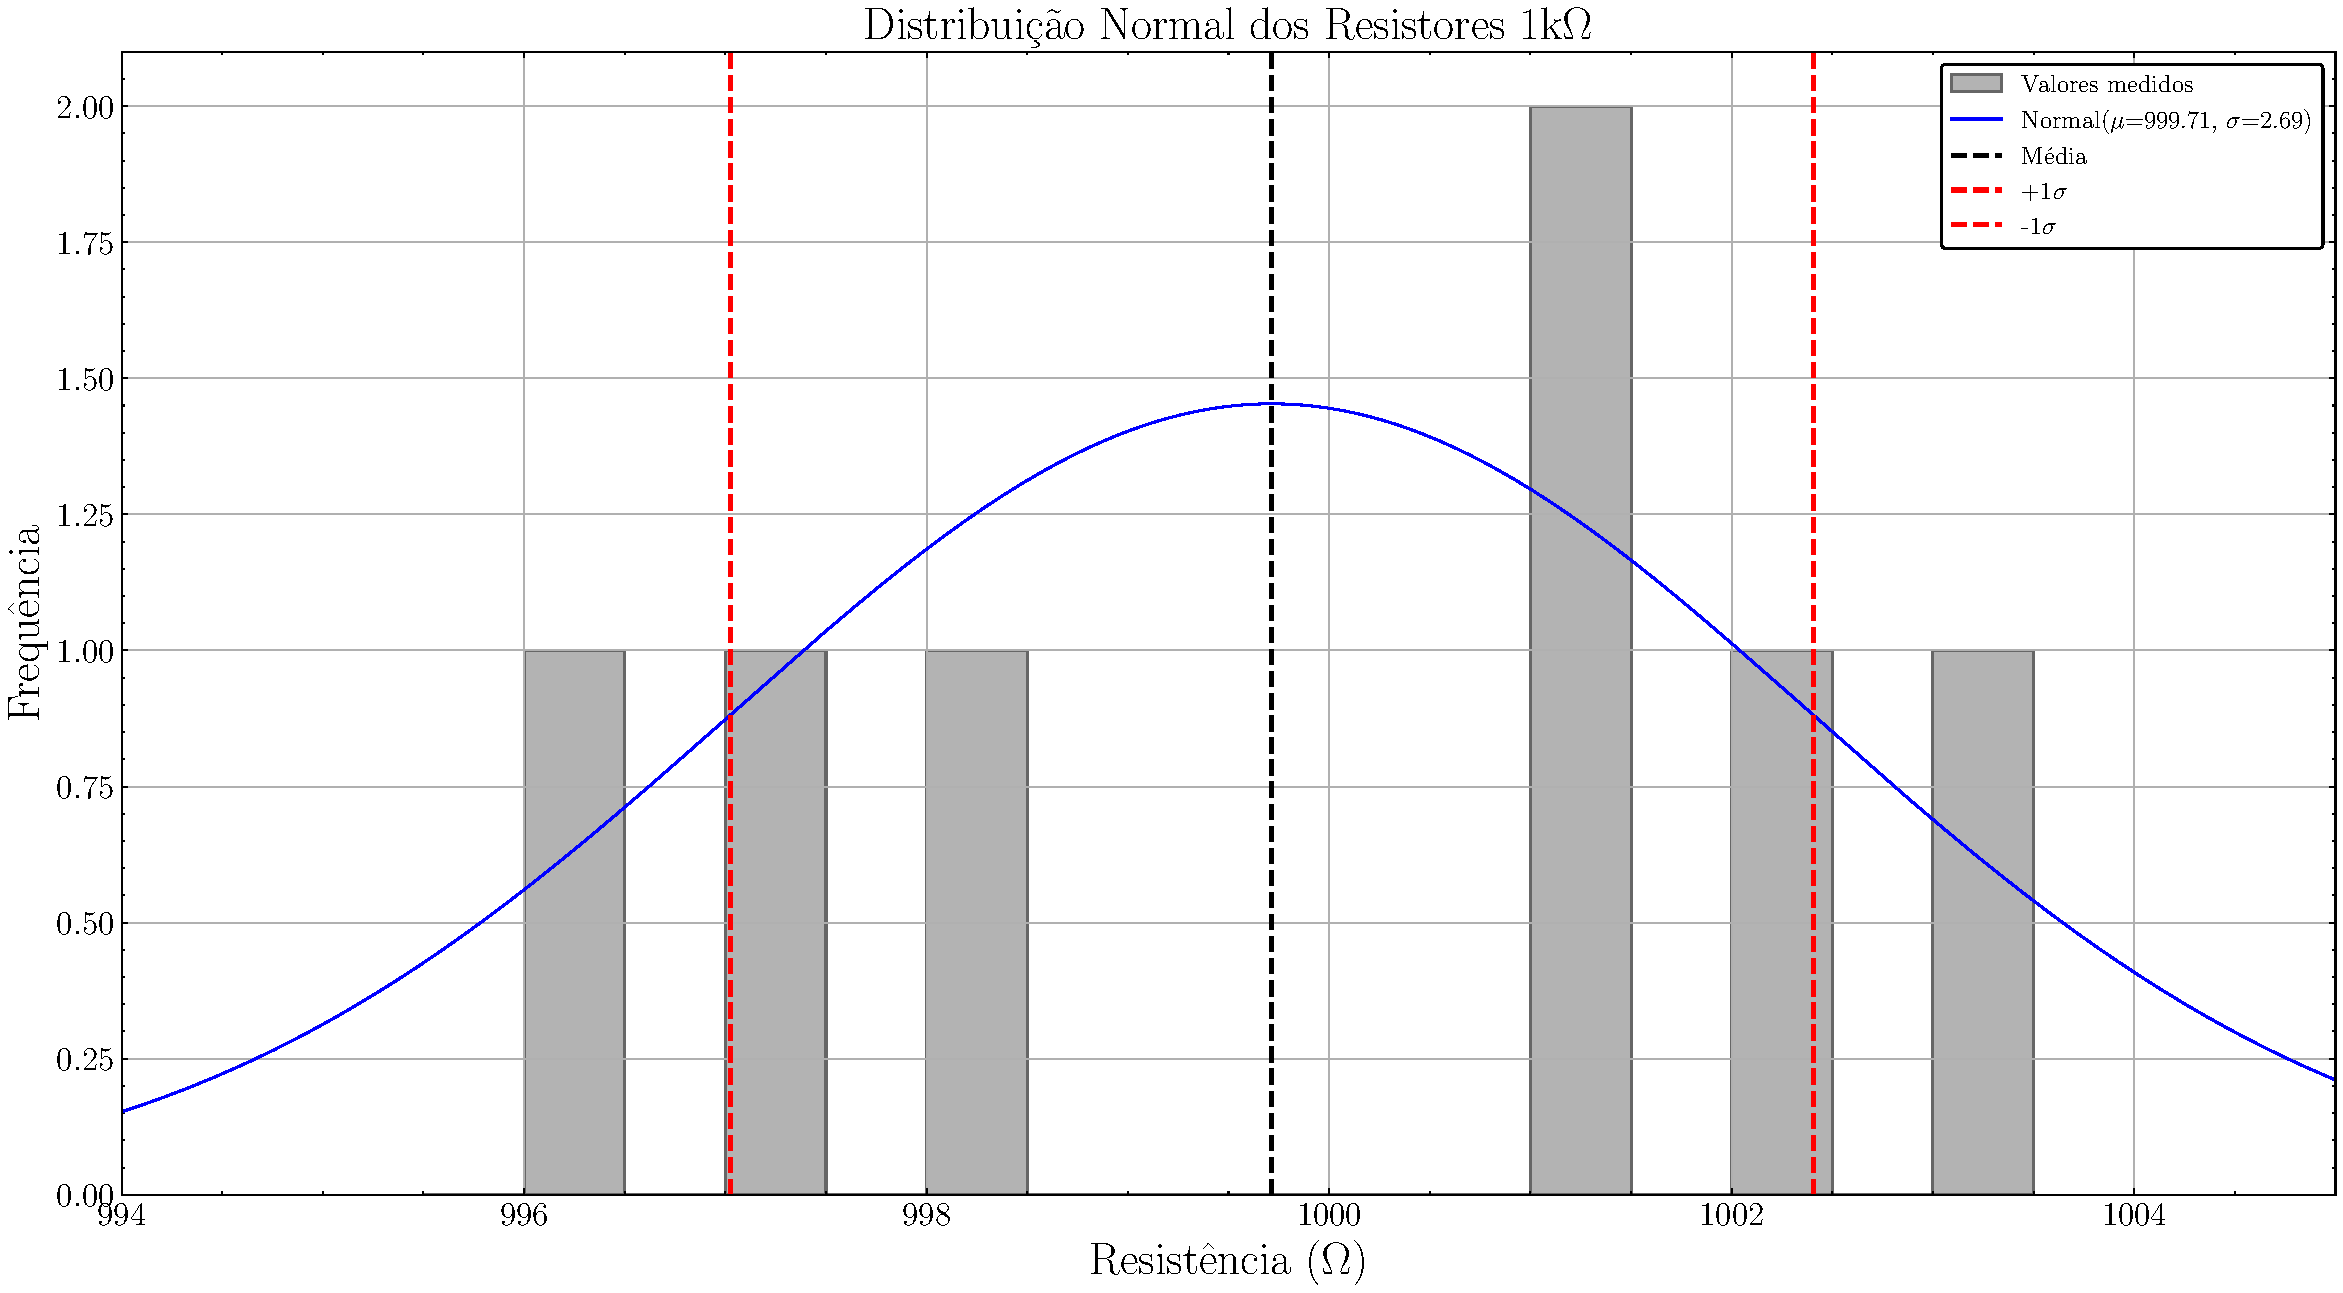
\includegraphics[width=0.8\linewidth]{figures/plot_hist_1k.pdf}
\end{figure}

\subsection{Associação de resistores (série, paralelo e mista):}

O erro absoluto na associação em série é: % [COMENTARIO PROFESSOR] qual a justificativa par o uso?

\begin{equation}
    \Delta R_{eq} = \sum_{i=1}^{n} \Delta R_i,
\end{equation}
\noindent
Onde $\Delta R_{eq}$: é a incerteza total $\Delta R_i$: são as incertezas individuais de cada resistor.

A propagação de erro para paralelo:

\begin{equation}
    \Delta R_{eq} = R_{eq}^2 \sqrt{\sum_{i=1}^{n} \left(\frac{\Delta R_i}{R_i^2}\right)^2},
\end{equation}

Onde $\Delta R_{eq}$: é a incerteza total da associação em paralelo.
- $\Delta R_i$: são as incertezas individuais de cada resistor.
- $R_{eq}$: é a resistência equivalente.



\begin{align*}
    \begin{split}
        R_{eq} & = 1k\Omega + \left(1M\Omega || 1k\Omega\right) + \left(1M\Omega || 1M\Omega\right) \\
               & + \left(1k\Omega || 1k\Omega\right) + 1M\Omega                                     % [COMENTARIO PROFESSOR] definir o significado do  operador de paralelo ||
    \end{split}
\end{align*}

\noindent
Podemos calcular a resistência equivalente das etapas do circuito misto, como mostrado abaixo

\begin{figure}[htbp]
    \centering
    \caption{Cálculo das resistências do circuito misto}
    \label{fig:plot_assoc_mista}
    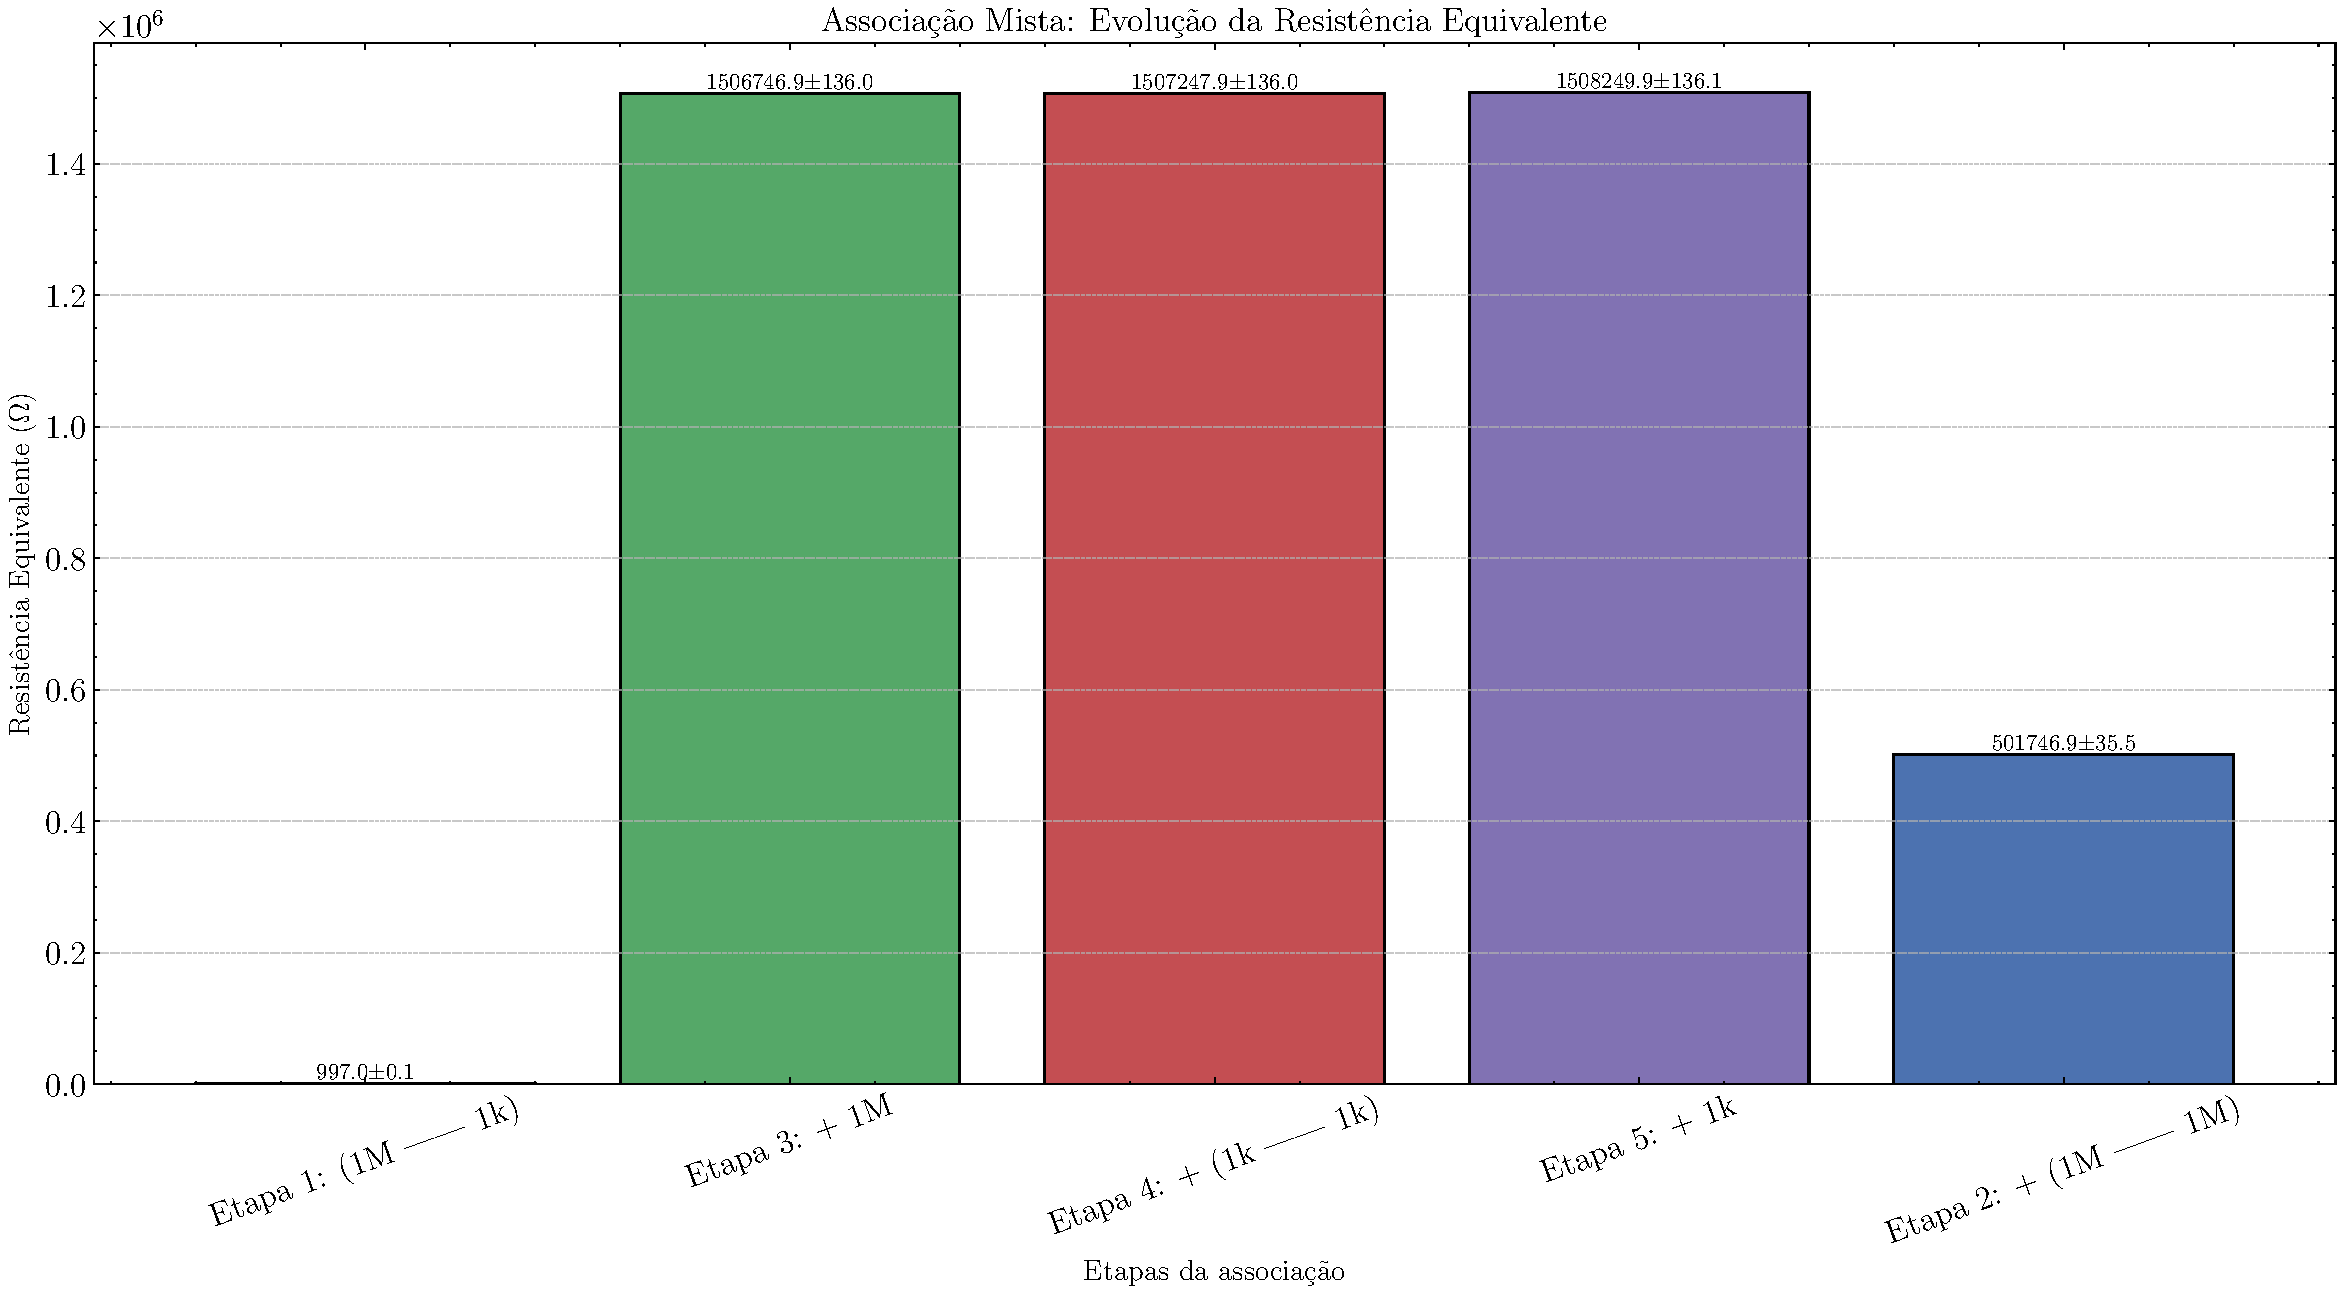
\includegraphics[width=0.8\linewidth]{figures/plot_assoc_mista.pdf}
\end{figure}

\section{Efeito Joule }

\subsection{Aquecimento de água}

O efeito Joule consiste na transformação da energia elétrica em energia térmica devido à passagem de corrente por um condutor ou resistor. Esse fenômeno é fundamental em aplicações como aquecedores elétricos, fusíveis, lâmpadas incandescentes e em muitos processos industriais.

No contexto deste experimento, investigamos o aquecimento de uma amostra de água quando submetida à dissipação de potência elétrica em um resistor submerso. O objetivo é analisar como a energia fornecida ao sistema é convertida em aumento de temperatura, levando em conta também as perdas térmicas para o ambiente.

A modelagem matemática do aquecimento é baseada na seguinte equação diferencial, que incorpora tanto o fornecimento de energia elétrica quanto a perda de calor para o ambiente (lei de Newton do resfriamento) % [COMENTARIO PROFESSOR] é resfriamento ou aquecimento?

\begin{equation}
    \frac{dT}{dt} = \frac{P}{mc} - k (T - T_"amb") % [COMENTARIO PROFESSOR] referenciar da onde essa equação veio
\end{equation}

\noindent
Onde

\begin{itemize}
    \item$T$: temperatura da água (em °C ou K)
    \item $P$: potência dissipada pelo resistor (em W)
    \item $m$: massa da água (em kg)
    \item $c$: calor específico da água (em J/kg·K)
    \item $k$: coeficiente de resfriamento para o ambiente (em $s^{-1}$)
    \item $T_"amb"$: temperatura ambiente (em °C ou K)
\end{itemize}

A solução numérica foi implementada de forma discreta, atualizando a temperatura a cada intervalo de tempo $d_t$:

\begin{equation}
    T_{i+1} = T_i + \left(\frac{P}{mc} - k (T_i - T_"amb")\right) d_t
\end{equation}

Onde $T_i$: temperatura no instante $i$, $d_t$: passo de tempo da simulação, medido em segundos.

Configuração experimental:
\begin{itemize}
    \item A potência $P$ foi calculada a partir da tensão e corrente aplicadas ao resistor.
    \item A massa $m$ da água e o calor específico $c$ são conhecidos.
    \item O coeficiente $k$ foi estimado a partir da taxa de resfriamento observada experimentalmente.
\end{itemize}

O gráfico a seguir apresenta a evolução da temperatura da água ao longo do tempo, mostrando tanto a curva teórica prevista pelo modelo quanto dados experimentais simulados. A diferença entre as curvas pode ser atribuída a fatores como perdas adicionais, imprecisão na medição de $k$ ou variações ambientais.

\begin{figure}[htbp]
    \centering
    \caption{Curva de aquecimento da água por efeito Joule}
    \label{fig:plot_temperatura}
    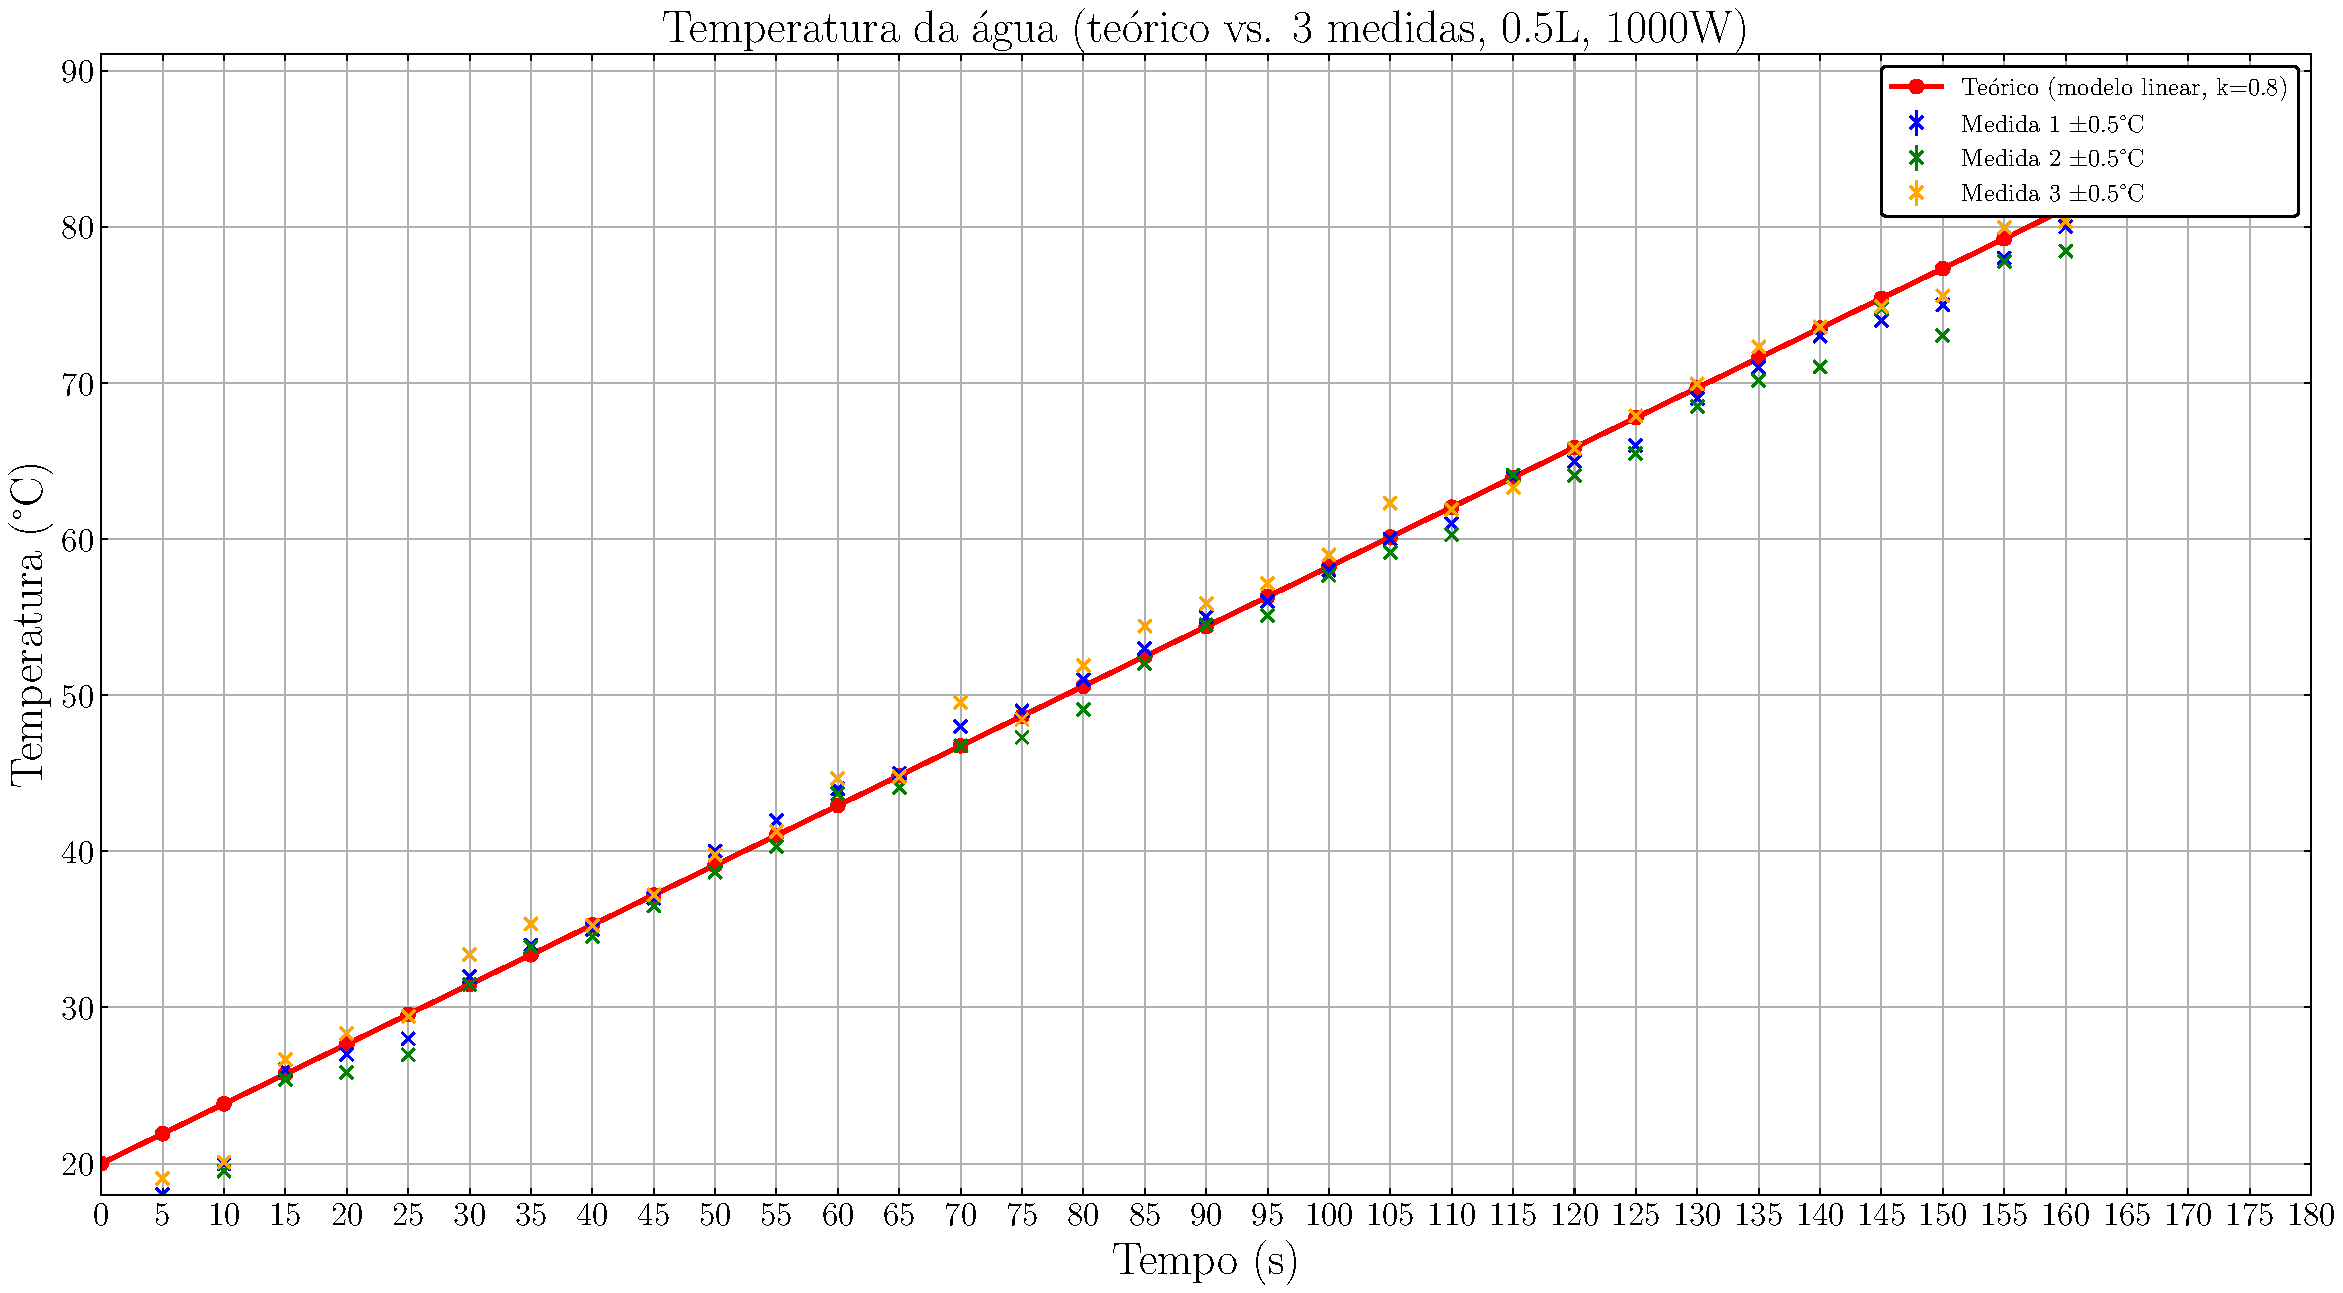
\includegraphics[width=0.8\linewidth]{figures/plot_temperatura.pdf}
\end{figure}

O estudo do efeito Joule é essencial para o dimensionamento seguro de dispositivos elétricos, evitando sobreaquecimento e otimizando a eficiência energética de sistemas de aquecimento.

\section{Conclusão:} % [COMENTARIO PROFESSOR] está muito pedagógico e pouco científico, quero ver a análise dos resistores e o efeito Joule

O experimento permitiu compreender, na prática, os princípios fundamentais das associações de resistores em série, paralelo e mista, bem como a influência dessas configurações na resistência equivalente de um circuito. As medições e análises estatísticas mostraram a importância de considerar as tolerâncias e incertezas dos componentes, reforçando a necessidade do cálculo de erros experimentais para uma avaliação precisa dos resultados.

A investigação do efeito Joule demonstrou como a energia elétrica é convertida em calor, evidenciando o papel dos resistores como elementos dissipadores. A modelagem matemática e a comparação com dados experimentais destacaram a relevância de fatores como perdas térmicas e transferência de calor para o ambiente, aspectos essenciais para o dimensionamento seguro de dispositivos elétricos.

Além de consolidar conceitos teóricos, o experimento proporcionou experiência com instrumentos de medição e análise de dados, habilidades essenciais para a formação em Engenharia. O estudo reforça a importância do rigor experimental e da análise crítica dos resultados, fundamentais para o desenvolvimento de soluções eficientes e seguras em projetos eletrônicos e sistemas de energia.

\end{document}
